% Use only LaTeX2e, calling the article.cls class and 12-point type.

\documentclass[11pt]{article}

\usepackage[round,semicolon]{natbib}
\usepackage{etoolbox}
\AtBeginEnvironment{quote}{\singlespacing\tiny}
% Use times if you have the font installed; otherwise, comment out the
% following line.

% added by SKH
%\usepackage{lineno}
%\linenumbers

\usepackage{times}
\usepackage{amssymb}
\usepackage{amsmath}

\usepackage[export]{adjustbox}

\usepackage{graphicx}
\graphicspath{ {images/} }

% for adjustwidth
\usepackage{changepage}

% The following parameters seem to provide a reasonable page setup.

\topmargin 0.0cm
\oddsidemargin 1cm
\textwidth 15cm 
\textheight 21cm
\footskip 1.0cm

\usepackage{newfloat}
\usepackage{amsmath}
\usepackage[labelfont=bf]{caption}
\usepackage{nameref}
\usepackage{rotating}
\usepackage{color}
\usepackage{float}
\renewcommand{\figurename}{{}}
\renewcommand{\thefigure}{{Figure~\arabic{figure}}}

\renewcommand{\tablename}{{}}
\renewcommand{\thetable}{{Table~\arabic{table}}}

\newfloat{suppfile}{thp}{losuppfile}
\renewcommand{\thesuppfile}{Supplementary~file~\arabic{suppfile}}
\floatname{suppfile}{}

\newfloat{suppfig}{thp}{losuppfig}
\renewcommand{\thesuppfig}{Supplementary~figure~\arabic{suppfig}}
\floatname{suppfig}{}

%
\newfloat{supptable}{thp}{losupptable}
\renewcommand{\thesupptable}{Supplementary~table~\arabic{supptable}}
\floatname{supptable}{}
%

\renewcommand{\theequation}{Equation~\arabic{equation}}

\newcommand\skhcomment[1]{{\color{cyan}[#1]}}
\newcommand\jdbcomment[1]{{\color{red}[#1]}}


\usepackage{hyperref}
\hypersetup{colorlinks,citecolor=blue,linkcolor=blue,urlcolor=blue}
\hypersetup{colorlinks,citecolor=blue,linkcolor=blue,urlcolor=blue}

\usepackage{seqsplit}

\usepackage{array}
\newcolumntype{P}[1]{>{\raggedright\arraybackslash}p{#1}}

\title{Experimentally informed site-specific substitution models deepen phylogenetic estimates of the divergence of viral lineages} 

\author
{Sarah K. Hilton$^{1,2}$  and Jesse D. Bloom$^{1,2}$\\
\\
\normalsize{$^1$Division of Basic Sciences and Computational Biology Program,}\\
\normalsize{Fred Hutchinson Cancer Research Center, Seattle, WA 98109, USA}\\
\normalsize{$^2$Department of Genome Sciences, University of Washington, Seattle, WA}\\
\normalsize{E-mail:  jbloom@fredhutch.org.}\\
}


% Include the date command, but leave its argument blank.

\date{}

\usepackage{setspace}
\onehalfspacing


\begin{document} 

% Make the title.

\maketitle 


\begin{abstract}
\noindent  
Molecular phylogenetics can be used to estimate the time since the divergence of modern gene sequences.
For highly diverged sequences, such phylogenetic techniques often estimate substantially more recent times than other methods.
In the case of viruses, there is independent evidence that the estimates of deep divergence times from molecular phylogenetics are too recent.
This discrepancy is caused in part by inadequate models of purifying selection leading to branch-length underestimation.
Here we show that models informed by experimental measurements of purifying selection due to site-specific amino-acid preferences lengthen deep branches on phylogenies of influenza virus hemagglutinin.
This deepening of branch lengths is due to more realistic stationary states of the models, and is independent of the branch-length-extension from modeling site-to-site variation in amino-acid substitution rate.
The branch-length extension from experimentally informed site-specific models is similar to that achieved by other approaches that allow the stationary state to vary across sites.
However, the improvements from these site-specific but time-homogeneous and site-independent models are limited by the fact that a protein's amino-acid preferences gradually shift as it evolves.
Overall, our work underscores the importance of modeling how site-specific purifying selection affects the stationary state when estimating deep divergence times---but also shows the inherent limitations of approaches that fail to model how site-specific functional constraints shift over time due to epistasis. 
\end{abstract}

\clearpage

\section*{Introduction} 
\skhcomment{from JDB: what is the "age" of a virus? Maybe "divergence time of viral lineages"}
skhcomment{from JDB: what is the less than a million actually? "Old" is not the right phrase.}
Estimating the divergence time of viral lineages of a virus is essential to understanding its evolutionary history, including its emergence, spread, and past zoonoses. 
This estimation is commonly done using the concept a ``molecular clock" to transform the branch lengths of the viral phylogenetic tree into age in years. 
However, this molecular dating technique often underestimates the age of many viruses, including measles, foamy virus, and ebola \skhcomment{(citations)}, compared to other methods which are independent of the viral phylogeny. 
For example, SIV (the original source of HIV) is estimated to be less than a million years old based on the viral phylogeny \citep{sharp2000origins,wertheim2009dating,worobey2010island} but estimated to be several million years old based on the host tree or endogenous retroviral elements  \citep{compton2013host} \skhcomment{(other citations)}. 
Overall, there is a systematic and substantially large underestimation of of branch length on viral phylogenies. 
\skhcomment{long branches}

Branch length underestimation is due, in part, to strong purifying selection masking the evolutionary signal in the observed sequences. 
Purifying selection can lead to mutational saturation, where multiple unobserved, substitutions occur at a single site along a long branch and erase the divergence signal \citep{holmes2003molecular}.
Furthermore, proteins do not have equal preference for all amino acids at all sites, this evident by a simple visual inspection of a multiple sequence alignment. 
How many and which amino acids tolerated at each site of the protein generate a site-specific expected rate of change. 
Failing to account for these site-specific constraints will lead to branch length underestimation. 
\skhcomment{you will have mutational saturation no matter what - this is a separate, addressable issue?}
\skhcomment{talk about the high mutation rate in viruses?}

Substitution models that incorporate site-to-site rate variation have been developed to decrease the bias in long branch estimation. 
The most common strategy is to allow a single rate-controlling parameter to vary according to some statistical distribution, such as a $\Gamma$-distributed $\omega$ (~dN/dS) \citep{yang2000codon}. 
This flexibility in the value of $\omega$ accounts for the site-to-site rate variation by allow some sites to have a higher dN/dS value than others. 
While this modification is simple and only requires the addition of one extra parameter, it does not describe site-specificity in its stationary state. 
That is, at evolutionary equilibrium, this model still assumes that each site in the protein evolves identically.  

An alternative approach is to model the site-specific amino-acid frequencies explicitly, such as those models in the mutation-selection family \citep{halpern1998evolutionary}. 
In these models, each amino-acid at each site in the protein is described by its own parameter and these differences are reflected in the stationary state of the model. 
The rate of change at a given site is controlled by these amino acid profiles and can now vary from site to site, as expected based on observations in nature. 
Importantly, these rate variations are not constrained to an arbitrary statistical distribution but by parameters with a direct biological interpretation. 

Mutation-selection models are presumably more biologically relevant but pose more practical challenges than the $\Gamma\omega$ models. 
These models are highly parametrized with 19 free parameters (the 20 amino acid preferences are constrained to sum to one) per site leading to thousands of parameters for the length of a normal protein. 
One way to avoid overfitting is to implement the model as a mixture model in either a bayesian \citep{lartillot2004bayesian} or maximum likelihood framework \citep{si2008empirical}. 

Alternatively, you can reduce the parameter space by defining the amino-acid frequencies \textit{a priori}. 
We have shown previously that we can define an Experimentally Informed Codon Model (ExpCM) \citep{bloom2014experimentally,bloom2014informed} from the mutation-selection family using measurements from deep mutational scanning \citep{fowler2014deep}, a high-throughput functional assay. 
ExpCM are therefore defined by amino-acid preferences measured in a \textit{single} genetic background and do not reflect any epistatic changes which may have occurred over the virus's evolutionary history. 
But they contain no more parameters than the traditional codon models while maintaining a site-specific stationary state. 
We hypothesize that the ExpCM will estimate longer branches than the traditional models due to the protein-specific description of purifying selection. 
\skhcomment{CAT model has been shown to work well (better) on saturated data.}

In order to test this hypothesis, we compared the branch lengths of a influenza virus HA phylogenetic trees optimized by different substitution models. 
We found that the ExpCM did extend the length of branches from the focal sequence on the tree \skhcomment{define focal} and that this extension was seen even in the context of $\Gamma$-distributed rate variation. 
Furthermore, we found this extension occurred even in the presence of $\Gamma$-distributed $\omega$, indicating that they are both important for modeling purifying selection. 
This supports the conclusion that modeling purifying selection, especially in a model with a non-uniform stationary state, is important to estimating the branch lengths on phylogenetic trees. 

\section*{Results and Discussion}

\subsection*{Different ways that substitution models account for purifying selection}

\begin{figure}
\centerline{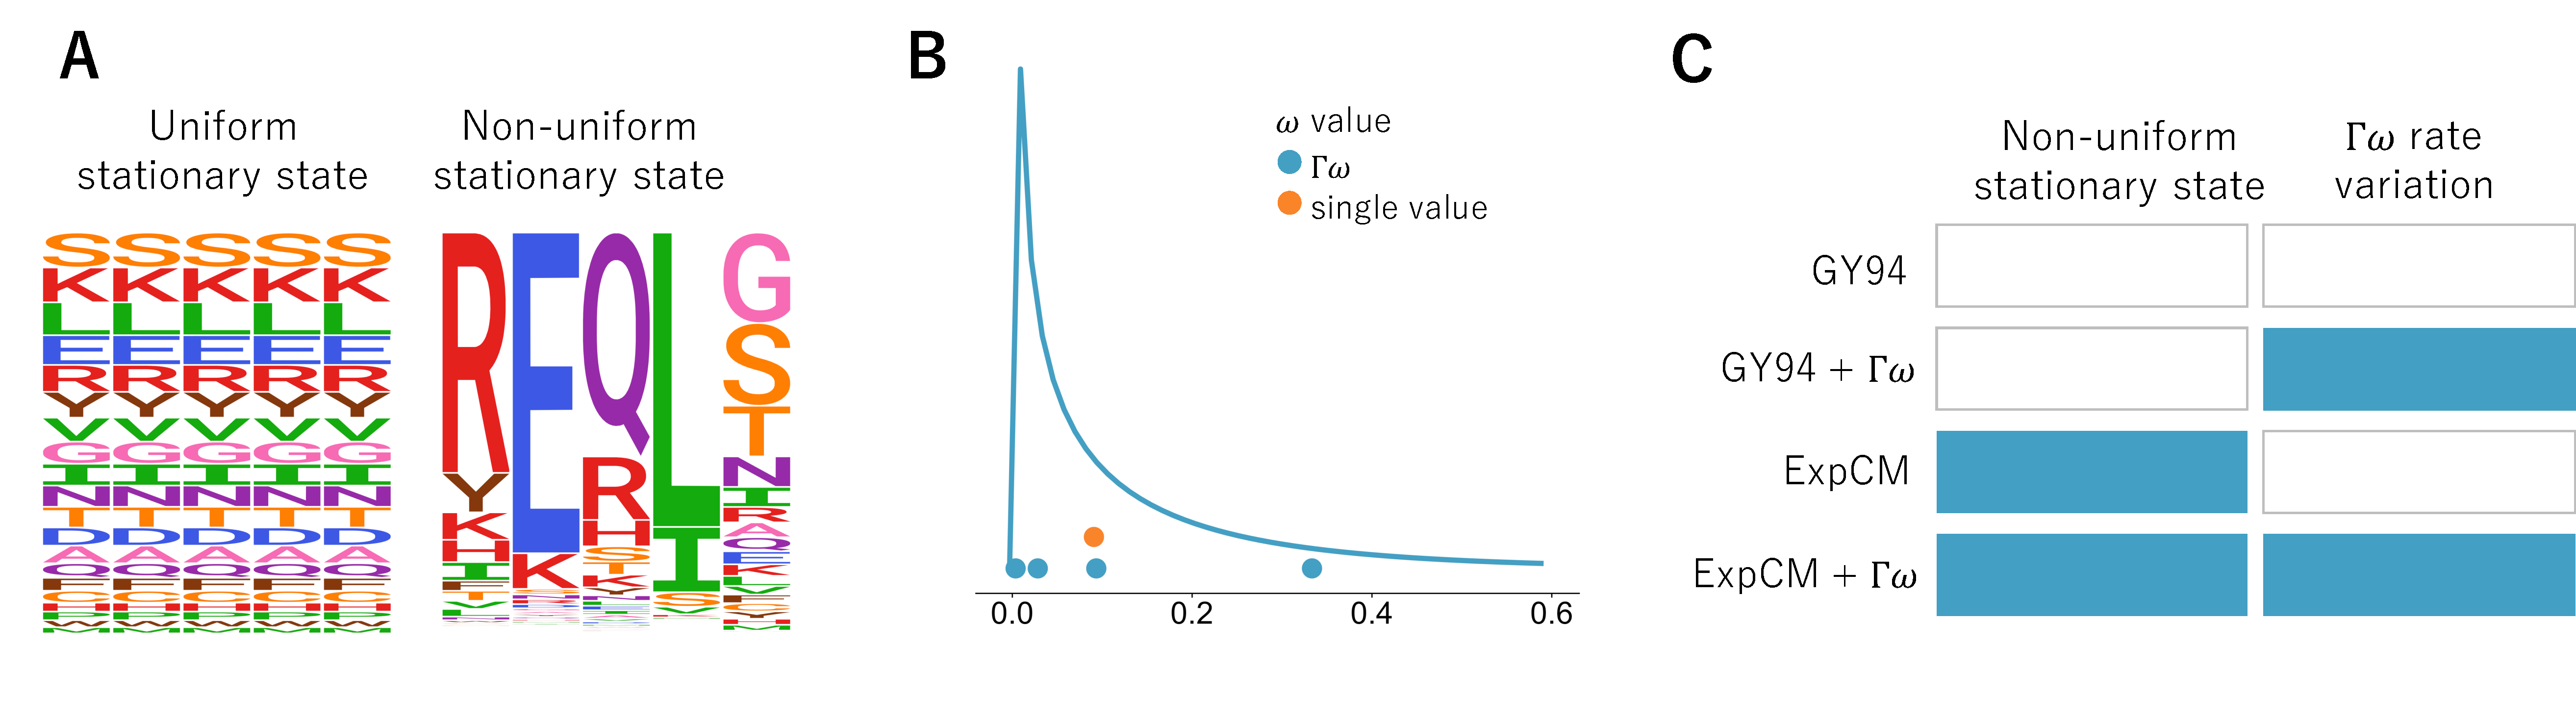
\includegraphics[width=0.90\textwidth]{figures/model_feature.pdf}}
\caption{\label{fig:model_feature}
\textbf{Different ways that codon models account for purifying selection.}
(A) The dN/dS parameter, $\omega$, can be defined as one gene-wide average (orange triangle) or allowed to vary according to some statistical distribution (blue circles). 
For computational tractability, the distribution is discretized into $K$ bins and $\omega$ takes on the mean of each bin~\citep{yang1994maximum,yang2000codon}. 
A gamma distribution ($\Gamma$) with $K=4$ bins is shown here.
(B) A substitution model stationary state defines the expected sequence composition after a very long evolutionary time. 
Most substitution models have stationary states that are uniform across sites.
However, substitution models can have site-specific stationary states.
In the logo plots, each column is a site in the protein and the height of each letter is the frequency of that amino acid at stationary state. 
(C) Substitution models can incorporate neither, one, or both of these features.
Here we will use substitution models from the Goldman-Yang~\citep[GY94;][]{goldman1994codon,yang2000codon} and experimentally informed codon model~\citep[ExpCM;][]{hilton2017phydms} families with and without gamma-distributed $\omega$ to represent all possible combinations.
}
\end{figure}

Proteins evolve under purifying selection to maintain their structure and function. 
This purifying selection is not homogenous across sites in a protein.
It is also not homogenous among the different amino acids at a given site.
For instance, some protein sites strongly prefer hydrophobic amino acids, others may be constrained to just one or a few amino acids, and yet others may tolerate many amino acids.
In general, these constraints are highly idiosyncratic among sites, and so pose a challenge for phylogenetic substitution models.

Here we consider how purifying selection is handled by codon models, which are the most accurate of the three classes (nucleotide, amino acid, and nucleotide) of phylogenetic substitution models in widespread use~\citep{arenas2015trends}.
Codon models distinguish between two types of substitutions: synonymous and nonsynonymous.
The relative rate of these substitutions is referred to as dN/dS or $\omega$.
In their simplest form, codon substitution models fit a single $\omega$ that represents the gene-wide average rate of fixation of nonsynonymous mutations relative to synonymous ones.
Here we will use such substitution models in the form proposed by \citet{goldman1994codon}.
When these models have a single gene-wide $\omega$ they are classified as M0 by \citet{yang2000codon}.
Here we will refer to M0 Goldman-Yang models simply as GY94 models. 
The gene-wide $\omega$ is usually $<1$~\citep{murrell2015gene}, and crudely represents the fact that many amino-acid substitutions are under purifying selection.

A single gene-wide $\omega$ ignores the fact that purifying selection is heterogeneous across sites.
The most common strategy to ameliorate this defect is to allow $\omega$ to vary among sites according to some statistical distribution~\citep{yang1994maximum,yang2000codon}.
For instance, in the M5 variant of the GY94 model~\citep{yang2000codon}, $\omega$ follows a gamma distribution as shown in \ref{fig:model_feature}A.
We will denote this model as GY94+$\Gamma\omega$.
A GY94+$\Gamma\omega$ captures the fact that the rate of nonsynonymous change can vary across sites. 
However, this formulation treats all nonsynonymous substitutions equivalently, since the rate is agnostic to the amino-acid identity of the mutation. 

A model formulation that accounts for the fact that purifying selection depends on the specific amino-acid mutation is provided by so-called ``mutation-selection'' models~\citep{halpern1998evolutionary,yang2008mutation,rodrigue2010mutation,tamuri2012estimating,mccandlish2014modeling}.
These models by explicitly define a different set of amino-acid preferences at each site in the protein. 
This more mechanistic formulation results in a site-specific stationary state (\ref{fig:model_feature}B). 
These models capture the site-to-site variation in amino-acid composition that is an obvious features of real proteins, and generally better describe actual evolution than models with only rate variation~\citep{lartillot2004bayesian, le2008phylogenetic, rodrigue2010mutation,hilton2017phydms,bloom2014experimentally}.

However, the increased realism of mutation-selection models comes at the cost of an increased number of parameters. 
Codon substitution models with uniform stationary states have only a modest number of parameters that must be fit from the phylogenetic data.
For instance, a GY94+$\Gamma\omega$ model with the commonly used F3X4 stationary state has 12 parameters: two describing the shape of the gamma distribution over $\omega$, a transition-transversion rate, and 9 parameters describing the nucleotide composition of the stationary state.
However, mutation-selection models must additionally specify 19 parameters defining the stationary state for \emph{each} site (there are 20 amino acids whose frequencies are constrained to sum to one).
This corresponds to $19\times L$ parameters for a protein of length $L$, or 9,500 parameters for a 500-residue protein.
It is challenging to obtain values for these parameters without overfitting the data~\citep{rodrigue2013statistical}.
Here we will primarily use experimentally informed codon models (ExpCM's)~\citep{bloom2014experimentally, hilton2017phydms, bloom2017identification} which define these parameters \textit{a priori} from deep mutational scanning experiments so they do not need to be fit from phylogenetic data.
The number of remaining free parameters for an ExpCM are similar to a non-site-specific substitution model.
Alternative strategies of obtaining parameters for site-specific stationary states via Bayesian \citep{lartillot2004bayesian, rodrigue2014site} or maximum-likelihood estimation~\citep{si2008empirical} are discussed in the last section of the Results.

Importantly, these two strategies for modeling purifying selection are not mutually exclusive.
Mutation-selection models such as ExpCM can still incorporate an $\omega$ parameter~\citep{haddox2017mapping}, which now represents the relative rate of nonsynonymous to synonymous substitution \emph{after} accounting for the constraints due to the site-specific stationary state.
This $\omega$ parameter for an ExpCM can be drawn from a distribution just like for GY94-style models. 
We will denote such models as ExpCM+$\Gamma\omega$.
\ref{fig:model_feature}C shows the full spectrum of models that incorporate all combinations of gamma-distributed $\omega$ and site-specific stationary states.

\subsection*{Effect of stationary state and rate variation on branch-length estimation}

\begin{figure}
\centerline{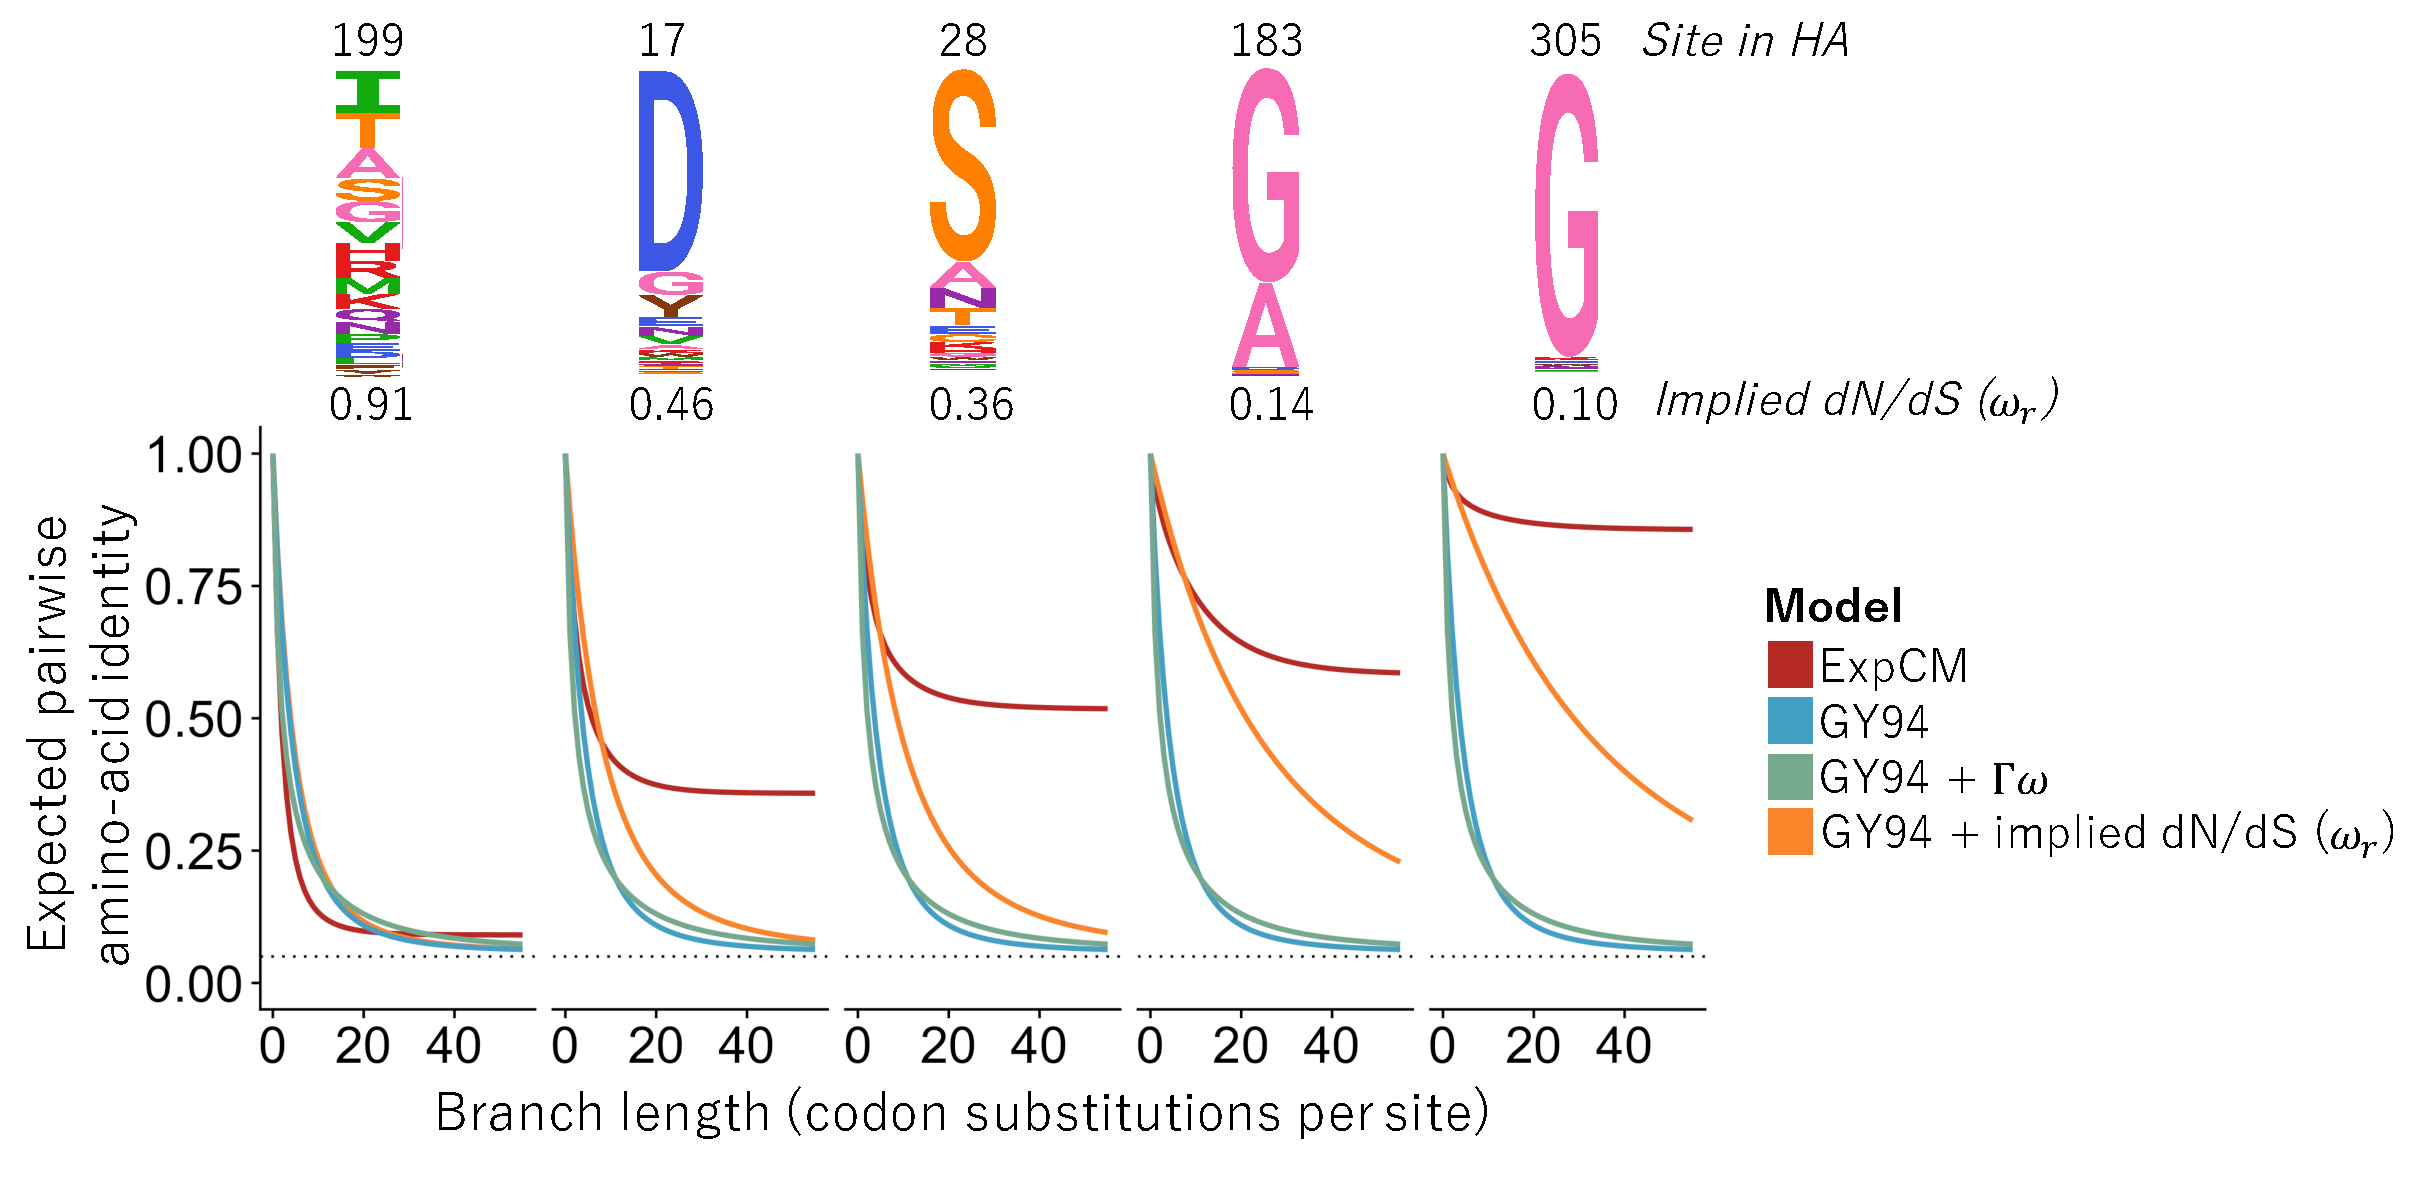
\includegraphics[width=0.90\textwidth]{figures/decay.pdf}}
\caption{\label{fig:decay}
\textbf{Effect of stationary state and $\Gamma\omega$ rate variation on predicted asymptotic sequence divergence.}
The logo plots at top show the amino-acid preferences for some sites in an H1 influenza hemagglutinin protein as measured by~\citet{doud2016accurate}.
The graphs show the expected amino-acid identity at that site for two sequences separated by a branch of the indicated length (\ref{eq:f}).
For the GY94 model, the graphs are identical for all sites since this models does not have site-specific parameters; the same is true for GY94+$\Gamma\omega$.
The graphs do differ among sites if we use the amino-acid preferences to calculate a different $\omega_r$ value for each site $r$ in a GY94 framework~\citep[\ref{eq:w_r};][]{spielman2015relationship}.
However, all GY94 models, including the one with site-specific $\omega_r$ values, approach the same asymptote since they all have the same stationary state.
But the ExpCM has different asymptotes for different sites since it accounts for how amino-acid preferences lead to site-specific stationary states.
}
\end{figure}

Given a single branch, a substitution model transforms sequence identity into branch length.
Under a molecular-clock assumption, this branch length is proportional to time.
The transformation from sequence identity to branch length is trivial when the sequence identity is high.
For instance, when where there has only been one substitution, then the sequence identity will simply be $\frac{L - 1}{L}$ for a gene of $L$ sites, and even a simple exponential model~\citep{zuckerkandl1965} will correctly infer the short branch length of $1/L$ substitutions per site.
However, as substitutions accumulate it becomes progressively more likely for multiple changes to occur at the same site.
In this regime, the accuracy of the substitution model becomes critical for transforming sequence identity into branch length.
Any time-homogenous substitution model predicts that after a very large number of substitutions, two related sequences will approach some asymptotic sequence identity.
For instance, if all 20 amino acids are equally likely in the stationary state, then this asymptotic sequence identity will be 0.05.
If the substitution model underestimates the asymptotic sequence identity then it will also underestimate long branch lengths, since it will predict that sequences that have evolved for a very long time should be more diverged than is actually the case.

\ref{fig:decay} shows how different substitution models predict sequence identity to decrease as a function of branch length for model parameters fit to a phylogeny of H1 influenza hemagglutinin (HA) genes.
The GY94 model predicts the same behavior for all sites, since it does not have any site-specific parameters.
This model predicts an asymptotic sequence divergence of \jdbcomment{?}, which is slightly higher than 0.05 since some of the 20 amino acids are favored due to more redundant codons and biases towards certain nucleotides.
Intuitively, this asymptotic sequence identity of \jdbcomment{?} seems low, since like many proteins HA has a highly conserved structure and function that imposes constraints that cause some sites to only sample a small subset of the 20 amino acids among all known HA homologs~\citep{nobusawa1991comparison}.

Accounting for site-to-site rate variation in GY94 models affects the rate at which the asymptotic sequence identity is approached, but not the actual value of this asymptote. 
For instance, \ref{fig:decay} shows that the GY94+$\Gamma\omega$ model takes longer to reach the asymptote than GY94, but the asymptote for both models is identical. 
This fact holds true even if we use experimental measurements of HA's site-specific amino-acid preferences~\citep{doud2016accurate} to calculate a different $\omega_r$ value for each site using the method of \citet{spielman2015relationship} (see \ref{eq:w_r}).
Specifically, this GY94+$\omega_r$ model predicts that different sites will approach the asymptote at different rates, but the asymptote is always the same (\ref{fig:decay}).
The invariance of the asymptotic sequence identity under different schemes for modeling $\omega$ is a fundamental feature of the mathematics of reversible substitution models.
These models are reversible stochastic matrices, which can be decomposed into stationary states and symmetric exchangeability matrices~\citep{nielsen2006statistical}.
The stationary state is invariant with respect to multiplication of the symmetric exchangeability matrix by any non-zero number.
Different schemes for modeling $\omega$ only multiply elements of the symmetric exchangeability matrix.
Therefore, no matter how ``well" a model accounts for site-to-site variation in $\omega$, it will always have the same stationary state as a simple GY94 model. 

However, mutation-selection models such as ExpCM's have site-specific stationary states.
Therefore, they predict that different sites will have different asymptotic sequence identities (\ref{fig:decay})---a prediction that accords with the empirical observation that some sites are much more variable than others in alignments of highly diverged sequences.
For instance, \ref{fig:decay} shows that at sites such as 348 and 305 in the H1 HA, an ExpCM but not a GY94-style model predicts that the divergence will always be low. 
When sites with highly constrained amino-acid preferences such as these are common, an ExpCM can estimate a long branch length at modest sequence identities that a GY94 model might attribute to a shorter branch.


\subsection*{Simulations demonstrate how failure to model site-specific stationary states leads to branch-length underestimation.}

\begin{figure}
\centerline{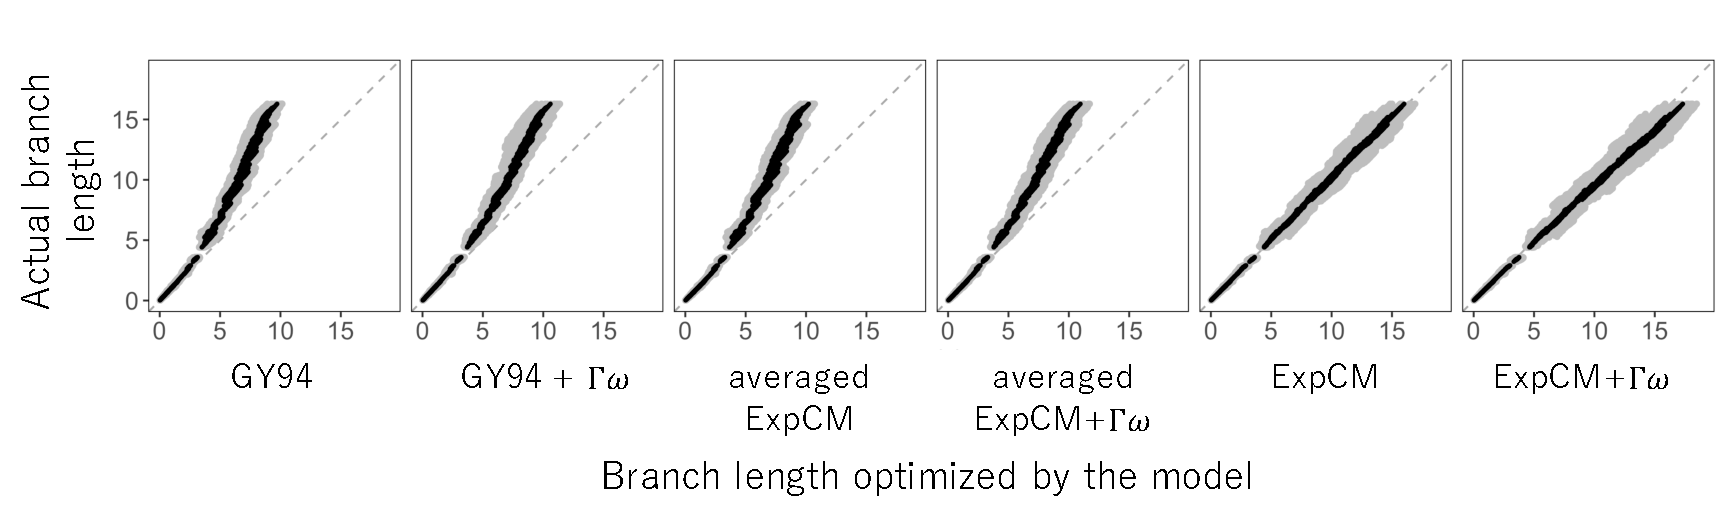
\includegraphics[width=0.85\textwidth]{figures/simulations}}
\caption{\label{fig:simulations}
\textbf{Branch lengths inferred on data simulated under a model with site-specific amino-acid preferences.} 
We simulated alignments along a phylogenetic tree of HA genes (see Figure~\ref{fig:empirical_trees}) using an ExpCM parameterized by the actual site-specific amino-acid preferences measured by deep mutational scanning of an H1 HA~\citep{doud2016accurate}.
We then inferred the branch lengths of this tree on the simulated alignments.
The inferred branch lengths for various models are plotted on the x-axis, and the actual branch lengths used in the simulations are on the y-axis.
We performed 10 simulations and inferences, and gray points show each inferred branch length from each simulation, and black points show the average of each branch length across simulations.
The grey dashed line at $y=x$ represents the behavior of an unbiased estimator. 
}
\end{figure}

To directly demonstrate the effect of stationary state and $\Gamma\omega$ rate variation on branch-length estimation, we tested the ability of a variety of models to accurately infer branch lengths on simulated data (\ref{fig:simulations}).
Specifically, we simulated alignments of sequences along the HA phylogenetic tree in \ref{fig:empirical_trees}) using an ExpCM parameterized by the amino-acid preferences of H1 HA as experimentally measured by deep mutational scanning~\citep{doud2016accurate}. We then estimated the branch lengths from the simulated sequences using all the substitution models in \ref{fig:model_feature}C, and compared these estimates to the actual branch lengths used in the simulations.

The models with a uniform stationary state underestimated the lengths of long branches separating the simulated sequences (\ref{fig:simulations}). 
The GY94 model estimated branches lengths which are only about 60\% of the true values for the longest branches. 
Accounting for site-to-site variation in $\omega$ did not fix the fundamental problem: the GY94+$\Gamma\omega$ did slightly better, but still substantially underestimated the longest branches.
However, there was no systematic underestimation of long branches by the ExpCM and ExpCM+$\Gamma\omega$ models, which accurately accounted for the site-specific amino-acid preferences used in the simulations.
The improved performance of the ExpCM's is due to their site-specific modeling of the stationary state: if we parameterize these models by site-specific amino-acid preferences that have been averaged across HA sites, then they perform no better than GY94 models.
Therefore, models with uniform stationary states are fundamentally incapable of accurately estimating the length of long branches in phylogenies of sequences that have evolved under strong site-specific amino-acid preferences.


\subsection*{Site-specific models estimate longer branches on real data.}

\begin{figure}
\centerline{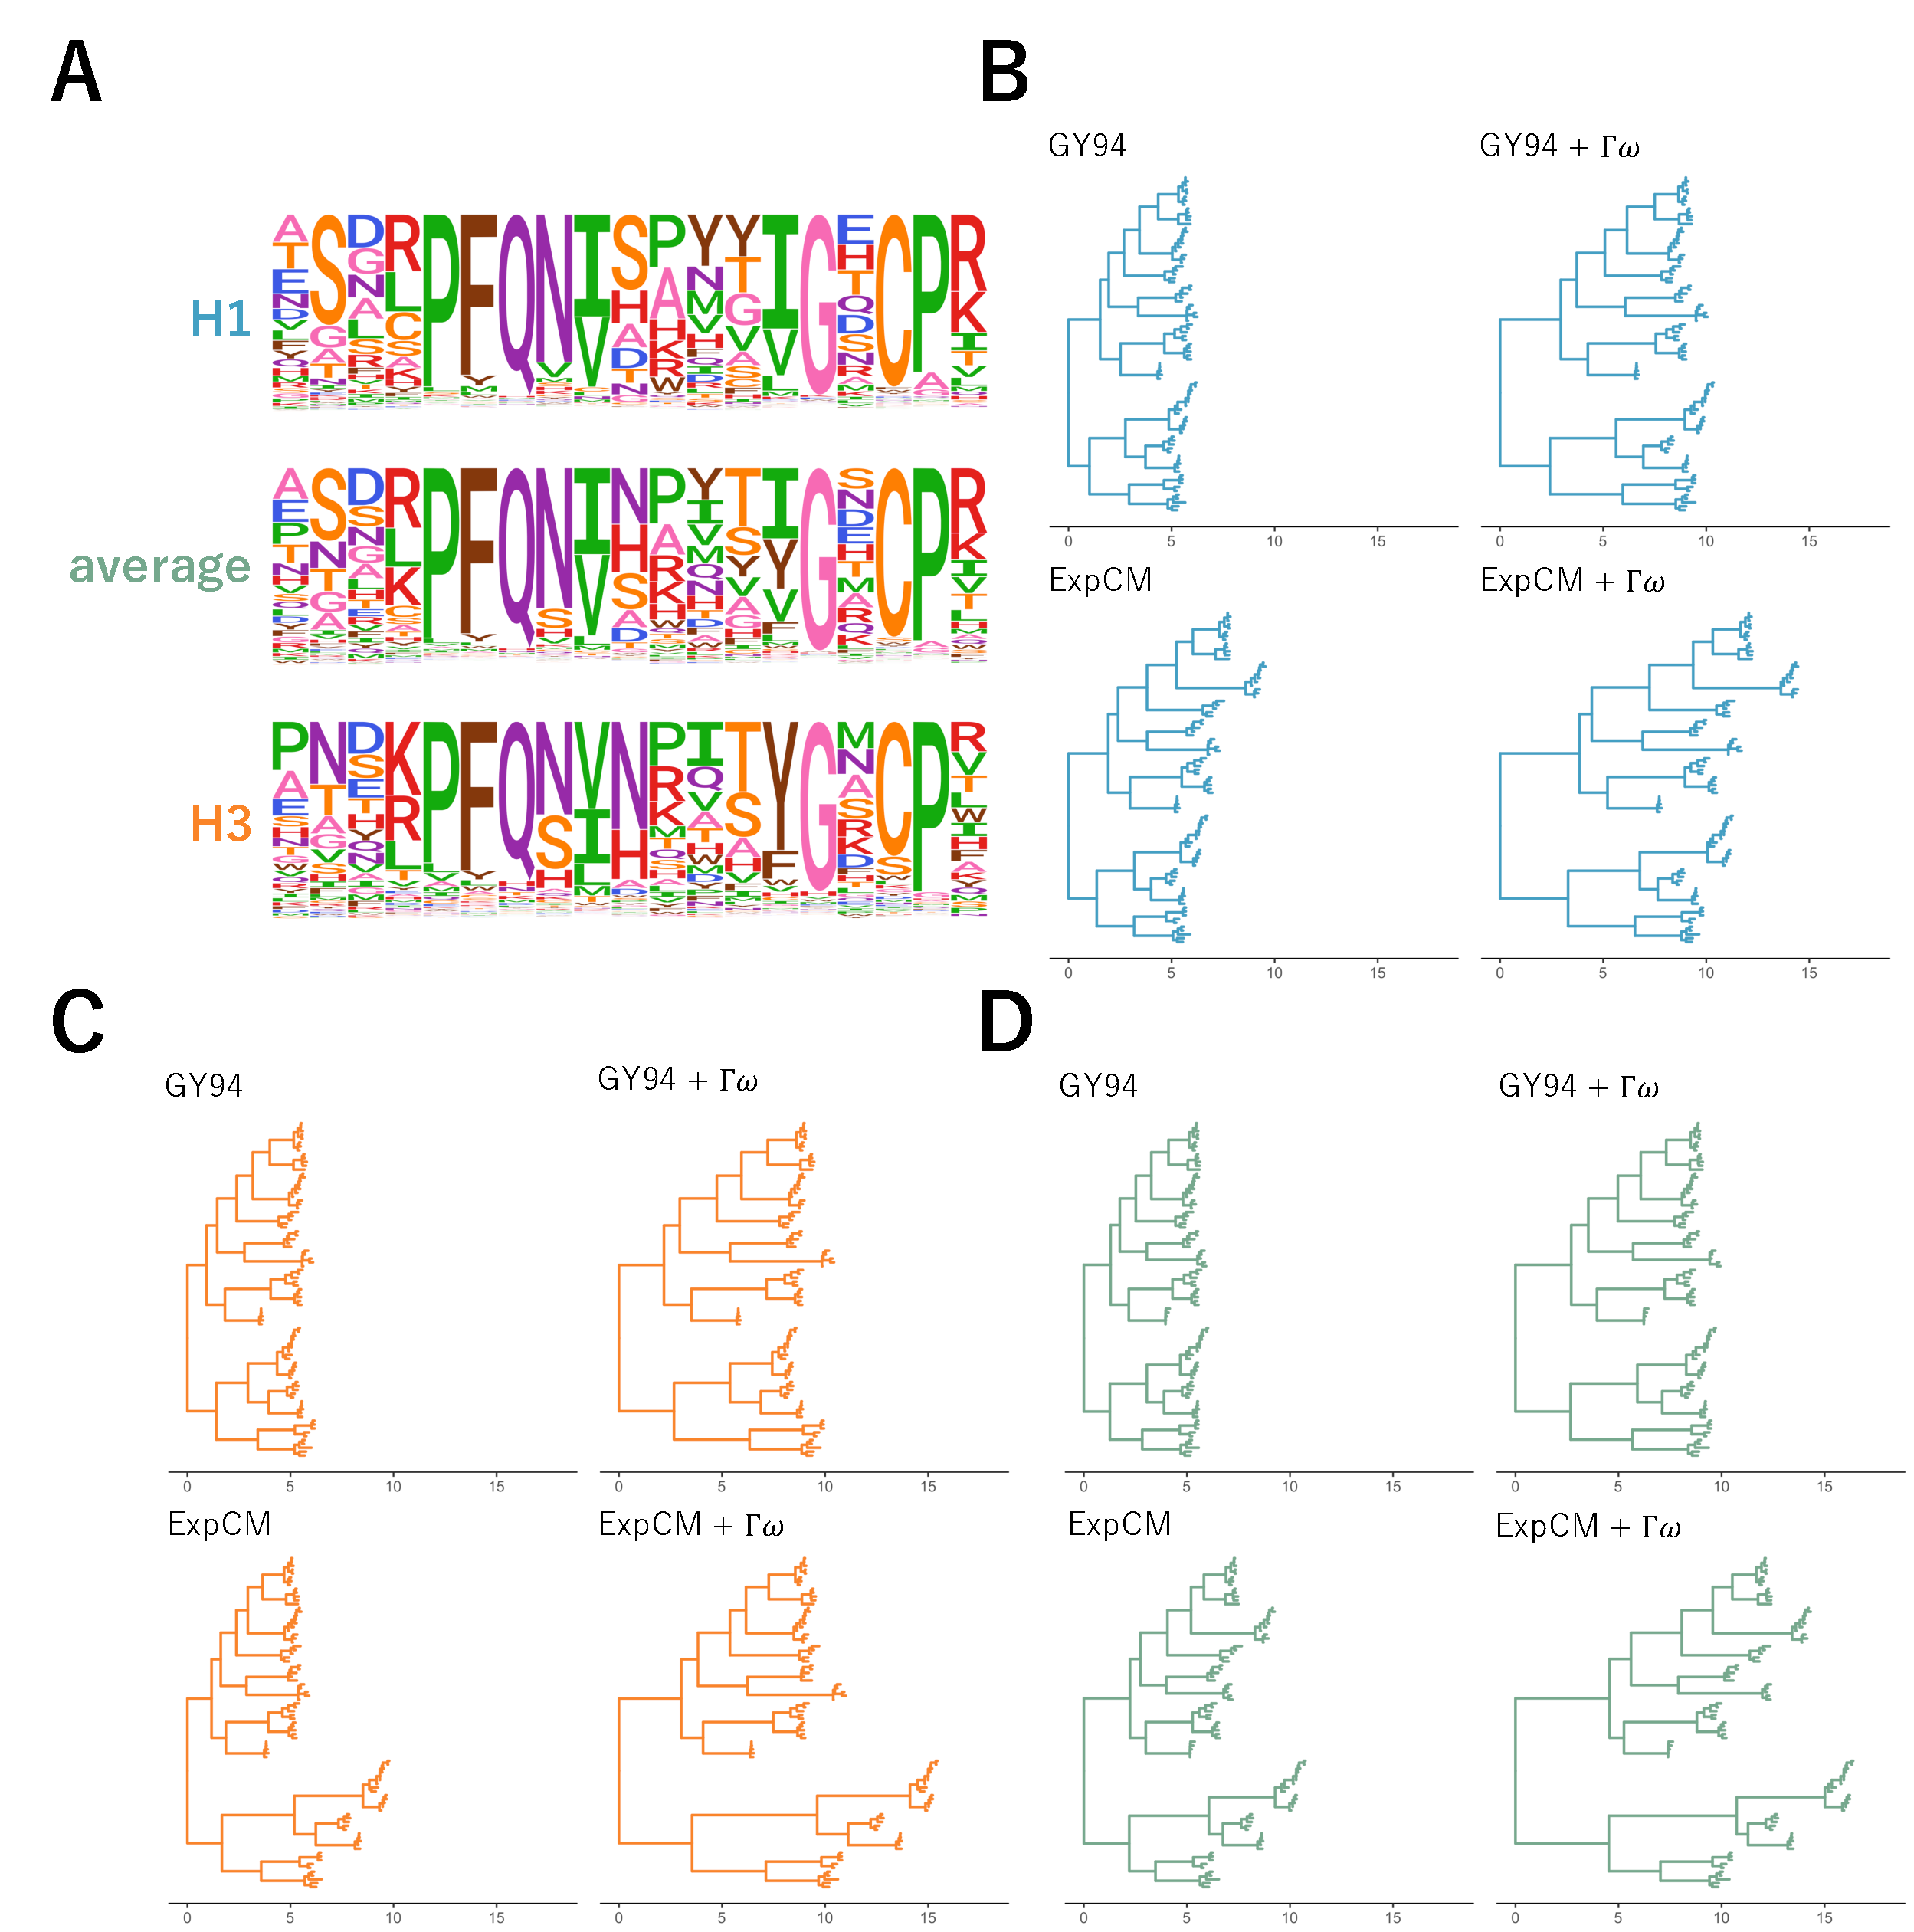
\includegraphics[width=\textwidth]{figures/empirical_trees.pdf}}
\caption{\label{fig:empirical_trees}
\textbf{Effect of site-specific stationary state and $\Gamma\omega$ rate variation on HA branch length estimation.} 
The branch lengths of the HA tree are optimized using the indicated ExpCM and GY94 models. 
The amino-acid preferences defining the model (ExpCM) or implied by the model (GY94) are shown as logoplots for 15 example sites in HA; the full set of experimentally measured amino-acid preferences defining each ExpCM are shown in \ref{suppfig:prefs_doud}, \ref{suppfig:prefs_lee}, and \ref{suppfig:prefs_average}. 
The ExpCM's use amino-acid preferences measured in deep mutational scanning of an H1 HA~\cite{doud2016accurate}, an H3 HA~\citep{lee2018deep}, or the average of the measurements for these two HAs.
The circle denotes the H1 clade and the triangle denotes the H3 clade. 
}
\end{figure}

\begin{table}[t!]
\caption{\label{tab:empirical_data}
{\bf Fitting of substitution models to the HA phylogenetic tree.}
The models fit here are the same ones in~\ref{fig:empirical_trees}. 
All ExpCMs describe the evolution of HA better than the GY94 models, as evaluated by the Akaike information criteria~\citep[$\Delta$AIC,][]{posada2004model}
The $\omega$ value for each of the $K=4$ bins is shown for the models with $\Gamma\omega$ rate variation. 
All ExpCM's fit a stringency parameter $>1$.
} 
     \begin{tabular}{cccccccccc}
        \hline
         Model & $\Delta$AIC & {\shortstack{Log\\ Likelihood}} & {\shortstack{$\omega$\\ (implied dN/dS)}} & {\shortstack{Stringency\\ parameter ($\beta$)}}\\ \hline
       	ExpCM + $\Gamma\omega$ (H1+H3 avg)  & 0 & -48751 & 0.19,  0.50,  0.90,  1.86 &  1.70\\
	ExpCM (H1+H3 avg)  &  950 & -49227 & 0.15 & 1.78\\
	ExpCM + $\Gamma\omega$ (H1)  & 1306 & -49404  & 0.13 ,  0.44,  0.91,  2.16 & 1.12\\
	ExpCM + $\Gamma\omega$ (H3) & 1737 & -49620 & 0.09,  0.33,  0.72,  1.77 & 1.28\\
	ExpCM (H1) & 2556 & -50030 &  0.13 & 1.22\\
	ExpCM (H3) &  3197 & -50350 & 0.12 & 1.45\\
	GY94 + $\Gamma\omega$  & 4719 & -51106 & 0.00,  0.03,  0.08,  0.26 & - \\
	GY94 & 7625 & -52560  & 0.07 & -\\
      \end{tabular}
\end{table}

The foregoing section shows the superiority of ExpCM's to GY94 models for estimating long branches on phylogenies simulated with ExpCM models.
But how do these models perform on real data?
Real genes do evolve under functional constraint, but these constraints are almost certainly more complex than what is modeled by an ExpCM.
However, if ExpCM's do a substantially better job than GY94 models of capturing the true constraints, then we might still expect them to estimate more accurate branch lengths.

To test the models on real data, we used actual sequences of influenza HA. 
The topology of HA phylogenetic trees (\ref{fig:empirical_trees}) makes these sequences an interesting test case for branch-length estimation.
HA consists of a number of different subtypes.
Sequences within a subtype have \jdbcomment{?} amino-acid identity, but sequences in different subtypes have as little as 38\% identity.
However, HA proteins from all subtypes (with the exception of an unusual subtype of bat influenza virus that we exclude from this analysis~\citep{zhu2013hemagglutinin,hoffmann2016hemagglutinin,sun2013bat}) have a highly conserved structure that performs a highly conserved function~\citep{ha2002h5,russell2004h1}.
We used \texttt{RAxML} with nucleotide model of substitution (GTRCAT) to infer a phylogenetic tree for 87 HA sequences drawn from 14 of the 18 subtypes (we excluded bat influenza and three other rare subtypes).
For the rest of this paper, we fix the tree topology to this \texttt{RAxML}-inferred tree.
Although the nucleotide model used with \texttt{RAxML} is probably less accurate than codon models, the modular subtype structure of the HA phylogeny means that most of the phylogenetic uncertainty probably lies in the length of the long branches separating the subtypes rather than in the tree topology itself.

There are two deep mutational scanning datasets for HA that estimated amino-acid preferences for all sites.
One scan measured the site-specific amino-acid preferences of an H1 HA~\citep{doud2016accurate} and the other measured the preferences of an H3 HA~\citep{lee2018deep}.
These two HAs have only $\sim$42\% amino-acid identity, and so are separated by a large distance on the phylogenetic tree (see triangle and circle on \ref{fig:empirical_trees}).
The experimentally measured amino-acid preferences clearly differ between the the H1 and H3 HA at a substantial number of sites~\citep[\ref{suppfig:prefs_doud}, 
\ref{suppfig:prefs_lee};][]{lee2018deep}.
Therefore, we also created a third set of amino-acid preferences by averaging the preferences measured in the deep mutational scanning of the H1 and H3 HAs, under the conjecture that these averaged preferences might do a better job of describing the ``average'' constraint on sites across the full HA tree.
These three sets of HA amino-acid preferences define three different ExpCM's.
 
We fit the GY94 model and each of the three ExpCM's to the fixed HA tree topology estimated using \texttt{RAxML}, and also tested a version of each of these models with $\Gamma\omega$ rate variation.
\ref{tab:empirical_data} shows that all of the ExpCM's fit the actual data much better than the GY94 model.
The best fit was for the ExpCM that was informed by the average of the H1 and H3 deep mutational scans.
For all models, incorporating $\Gamma\omega$ rate variation improved the fit, although even ExpCM's without $\Gamma\omega$ greatly outperformed the GY94+$\Gamma\omega$ models.
As mentioned in the previous section, $\omega$ is generally fit to values $<1$ in phylogenetic studies~\citep{murrell2015gene} and our results follow this trend. 
\ref{tab:empirical_data} shows that most models were fit to very small $\omega$ values. 
However, the ExpCM's always fit $\omega$ values greater than the GY94 model and the ExpCM's with $\Gamma\omega$ all have one $\omega >1$. 
This increase in $\omega$ values makes sense due to the different interpretation of $\omega$ in each family of models. 
The ExpCM $\omega$ is the relative rate of fixation of nonsynonymous to synonymous mutations \textit{after} accounting for the functional constraints described by the deep mutational scanning amino-acid preferences.
The ExpCM's more realistic null model gives it more power to detect diversifying selection, such as the \skhcomment{obvious} immune pressure on HA~\citep{bloom2017identification}. 

\ref{fig:empirical_trees} shows that modeling purifying selection via either $\Gamma\omega$ rate variation or a site-specific stationary state increases the estimated branch lengths.
But important, the effects from these two methods of modeling purifying selection are largely independent.
For every model (GY94 or any of the three ExpCM's), the $\Gamma\omega$ version estimates longer deep branches.
In addition, all ExpCM's estimate longer deep branches than the GY94 model, and all ExpCM+$\Gamma\omega$ models estimate longer deep branches than the GY94+$\Gamma\omega$ model.

However, while adding $\Gamma\omega$ rate variation increases the length of deep branches in a fashion that appears roughly uniform across the tree (\ref{fig:empirical_trees}), the branch lengthening from the ExpCM's is not uniform across the tree. 
In particular, the branch lengthening is most pronounced near the sequence of the HA that was used in the deep mutational scanning experiment that parameterized the ExpCM.
For instance, the ExpCM informed by the H1 data most dramatically lengthens branches near the H1 clade of the tree, while the ExpCM informed by the H3 data has the largest effect on branches near the H3 clade.
The ExpCM informed by the average of the H1 and H3 data has a more uniform effect, but still most strongly affects branches near either the H1 or H3 clades.
Therefore, \ref{fig:empirical_trees} shows that the ExpCM's estimate longer branches but that the effect is clearly biased by the given set of preferences used to define the model.

\subsection*{Competing effects of shifting preferences and long branches.}

\begin{figure}
\centerline{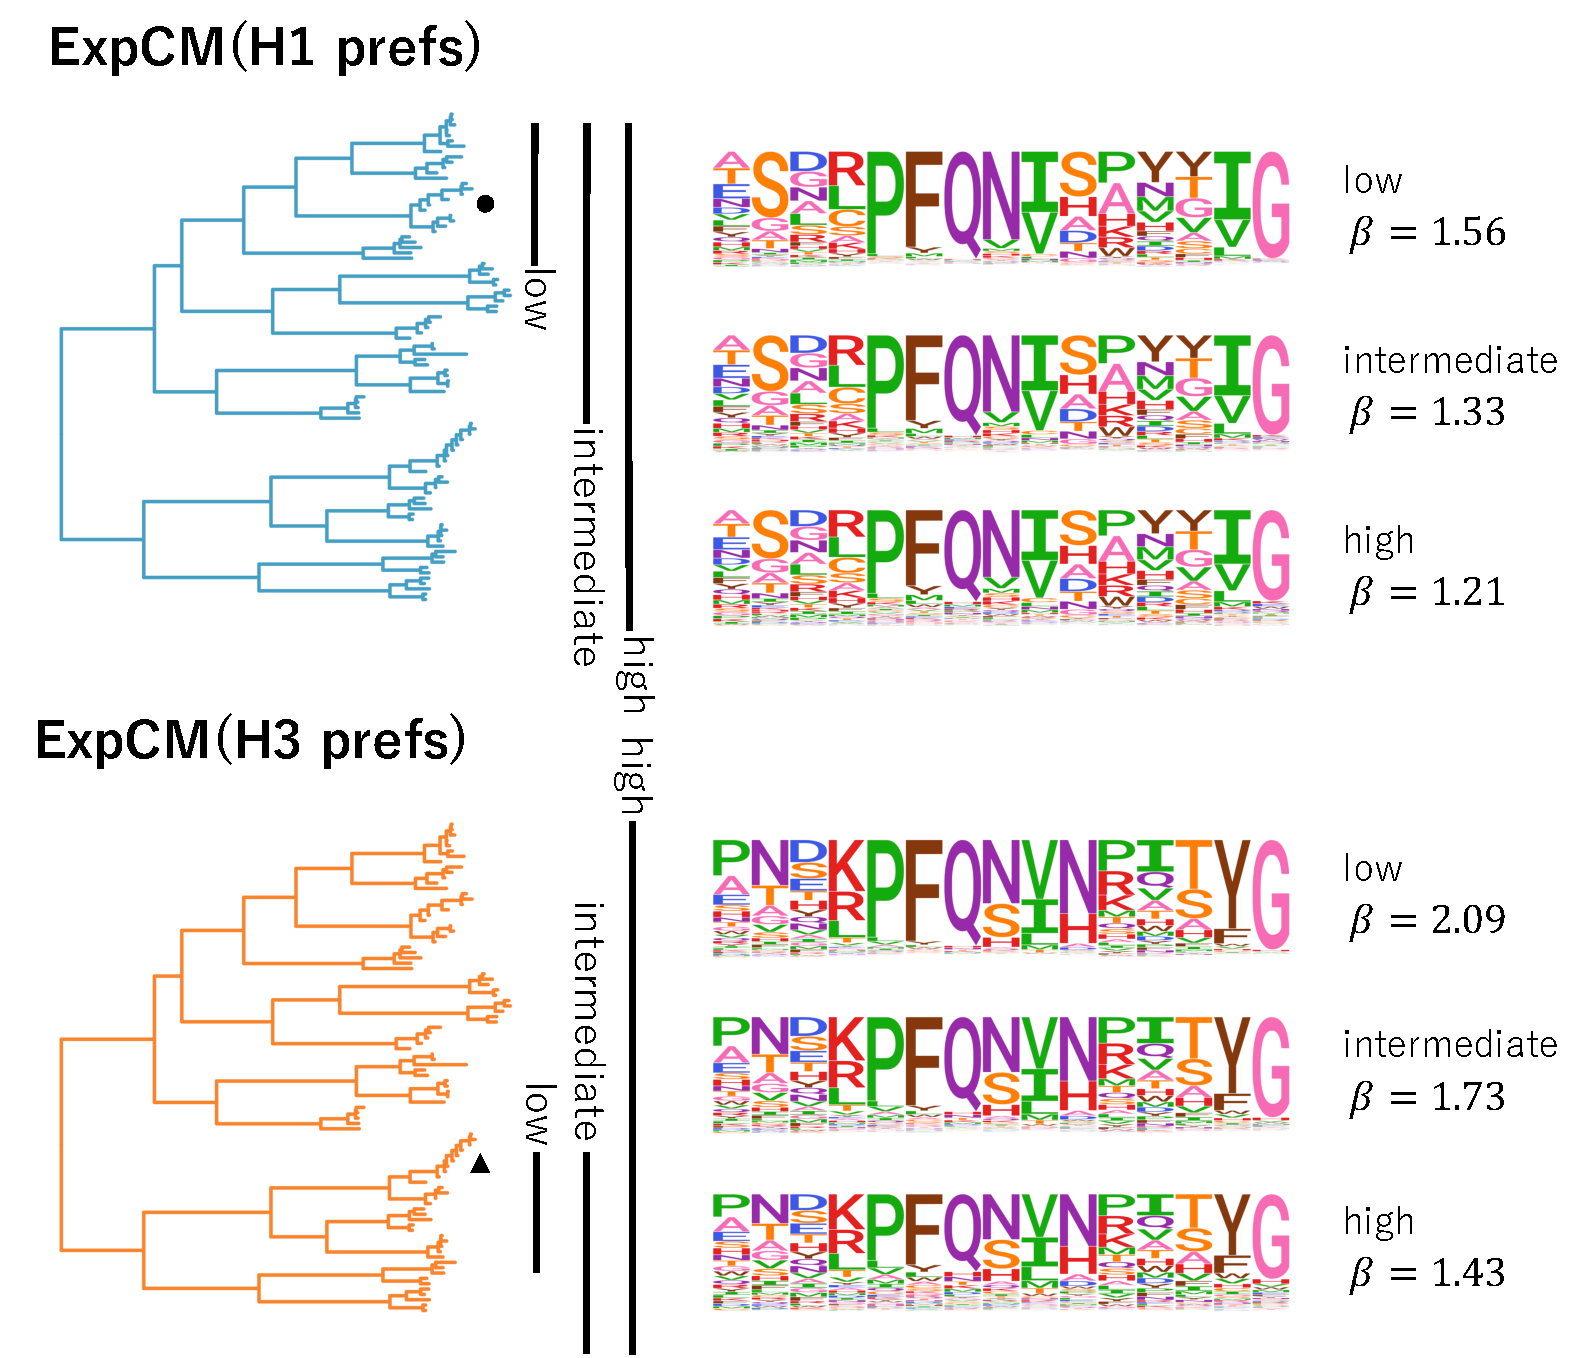
\includegraphics[width=0.75\textwidth]{figures/compete}}
\caption{\label{fig:compete}
\textbf{The congruency between natural selection and the deep mutational scanning measurements decreases with sequence divergence.} 
We fit an ExpCM informed by the H1 or H3 deep mutational scanning experiments to trees spanning sequences with low, intermediate, and high divergence from the sequence used in the experiment. 
The ExpCM stringency parameter ($\beta$) is a measure of the congruency between natural selection and the experimental measurements. 
Larger values of $\beta$ indicate that natural selection prefers the same amino acids as the experiments but with greater stringency. 
As divergence increases between the HA used in the experiment and the other sequences in the tree, the $\beta$ value decreases.
Therefore, the preferences measured in each experiment are progressively less congruent with those of the HA sequences on the tree as we include increasingly diverged sequences. 
}
\end{figure}

The fact that an ExpCM has the greatest effect on branches close to the sequence used in the experiment can be rationalized in terms of existing knowledge about how epistasis shifts protein amino-acid preferences during evolution~\jdbcomment{Stokes shift paper, Shah et al paper, Doud et al 2015, Haddox et al 2018, look at other papers cited about Stokes shift in Haddox et al 2018}.
In reality, sites in proteins do not have completely conserved site-specific amino-acid preferences. 
Rather, the effect of a mutation at one site in a protein can depend on the amino-acid identity of other sites in the protein~\jdbcomment{Maybe cite a couple of general papers on epistasis, some good ones in Haddox et al 2018}. 
The deep mutational scanning experiments that inform our ExpCM's are each done in the context of a single HA genetic background, and so do not account for how such epistatic interactions can cause amino-acid preferences to shift as substitutions accumulate. 
Therefore, it makes sense that an ExpCM would most accurately describe the site-specific amino-acid preferences of sequences closely related to the one used in the experiment.
 
We can observe this phenomenon of shifting amino-acid preferences degrading the accuracy of the ExpCM by fitting trees containing increasingly diverged sequences.
Specifically, for each HA for which we have deep mutational scanning data, we created three HA phylogenetic trees: a ``low'' divergence tree that contains only sequences with \skhcomment{$\ge ?$} amino-acid identity to the HA used in the experiment, an ``intermediate'' divergence tree that contains sequences with \skhcomment{$\ge ?$} amino-acid identity to the HA in the experiment, and a ``high'' divergence tree that contains all the HAs (which have as little as 38\% identity to the HA in the experiment).
\ref{fig:compete} shows these sets of HA sequences.
For each of the subtrees in \ref{fig:compete}, we examined the congruence between site-specific natural selection over the tree and the amino-acid preferences measured in the deep mutational scanning experiment. 
We used the ExpCM fit parameter $\beta$ to measure this congruency~(\ref{eq:Frxy}). 
In essence, $\beta$ rescales the deep mutational scanning measurements~(\ref{fig:compete}). 
Larger values of $\beta$ indicate that natural selection prefers the same amino acids as the experiments but with a greater stringency, or a strong congruence between natural selection and the experimental preferences. 

\ref{fig:compete} shows that as the divergence from the sequence used in the deep mutational scan increases, the value of $\beta$ decreases. 
This inverse relationship between $\beta$ and overall divergence is seen for the ExpCM's informed by both the H1 and H3 experiments.
Specifically, as the $\beta$ value decreases, the preferences ``flatten" and draw less information from the experiment. 
At the most extreme, $\beta = 0$, the preferences would be perfectly uniform and look identical to the GY94 preferences in \ref{fig:empirical_trees}. 
The flattening with increasing sequence divergence arises because the amino-acid preferences are increasingly less accurate as we move away from the experimental sequence on the tree.
As shown in \ref{fig:simulations}, the ability of models with site-specific stationary states to extend branch lengths requires these stationary states to be accurate\jdbcomment{Maybe expand the simulation figure to have two rows and have something with randomized preferences too}.
This fact also helps rationalize why the ExpCM defined by the average of the H1 and H3 experiments, representing the ``average" constraint on HA, does better across the whole tree (\ref{fig:empirical_trees}). 
 
The fact that amino-acid preferences shift as proteins evolve leaves us with an inherent tension: models with site-specific stationary states only become important for accurate branch-length estimation as sequences become increasingly diverged, but this same divergence degrades the accuracy of extrapolating the amino-acid preferences from any given experiment across the phylogenetic tree.
More importantly, the fact that amino-acid preferences shift over time means that there will not be any model with a single set of site-specific stationary states that accurately describes a phylogenetic tree that covers a wide span of sequences.

\subsection*{Models with stationary states estimated from natural sequences give similar results to ExpCM's}

\begin{figure}
\centerline{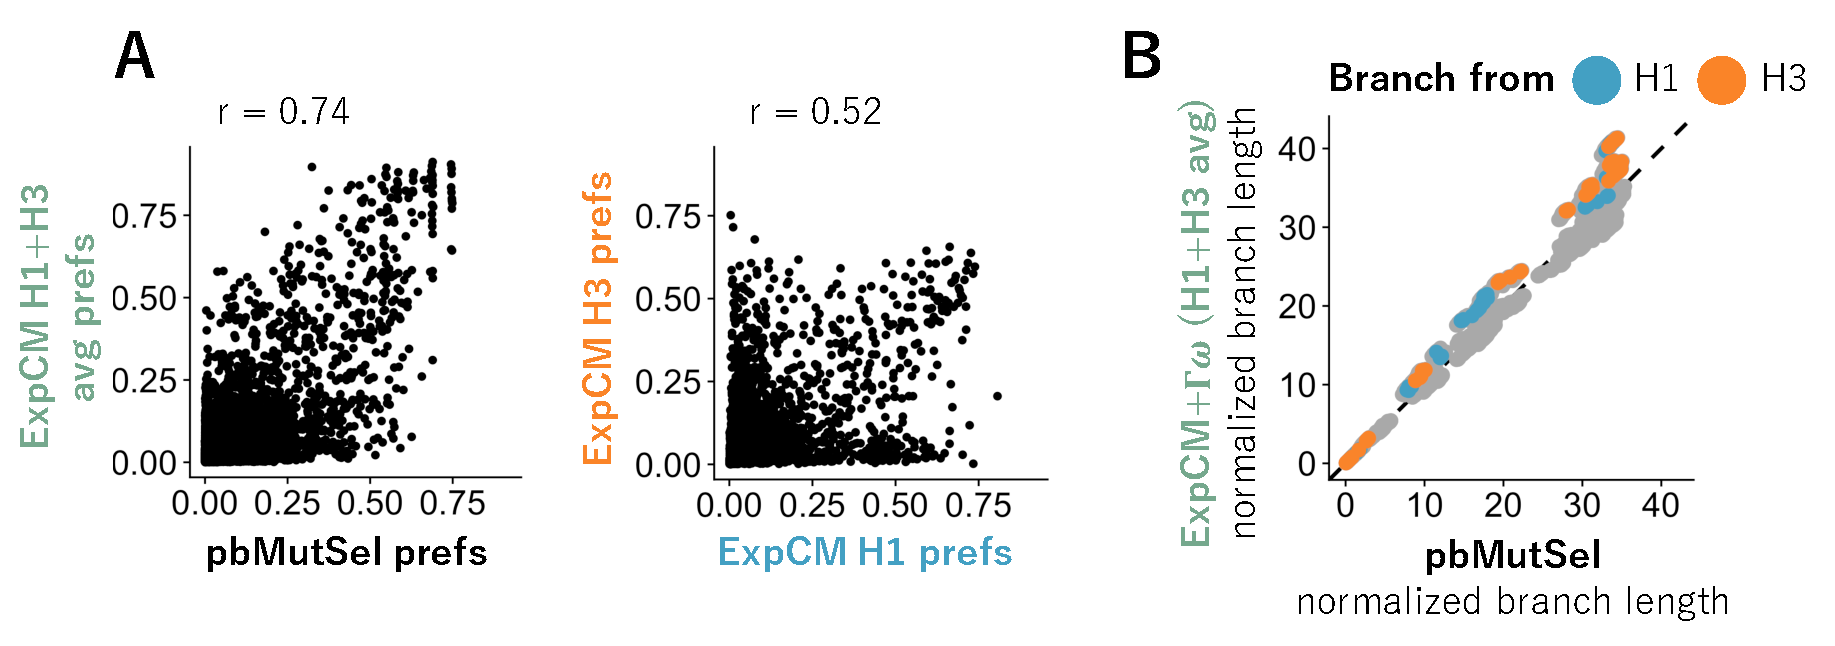
\includegraphics[width=0.99\textwidth]{figures/phylobayes.pdf}}
\caption{\label{fig:phylobayes}
\textbf{Comparison of ExpCM and \texttt{phylobayes}}
We estimated the branch lengths of the HA tree in \ref{fig:empirical_trees} using the mutation-selection model implemented in \texttt{phylobayes}. 
In comparison to ExpCM's, the \texttt{phylobayes} model infers the site-specific amino-acid preferences from the phylogenetic data rather than defining them \textit{a priori} from deep mutational scanning experiments. 
\skhcomment{I am less sold on using colors on the x or y axis. Is it too confusing with the focal sequence color coding in panel B}
}
\end{figure}

The previous sections used ExpCM's, which are mutation-selection models that use site-specific amino-acid preferences that have been measured experiments.
However, there are other implementations of mutation-selection models that infer the amino-acid preferences from natural sequence data.
These models are generally implemented in a Bayesian framework, which avoids the overfitting problems associated with trying to make maximum-likelihood estimates of thousands of parameters giving the site-specific stationary states.
For example, the CAT model~\citep{si2008empirical} implements site-specific stationary states for amino-acid substitution models by drawing the stationary state at each site from a mixture model of distinct, finite amino-acid profiles \jdbcomment{wording in preceding sentence might need some tweaking}.
However, the model most comparable to our ExpCM's is the mutation-selection model implemented in \texttt{phylobayes}, \jdbcomment{and referred to as MutSel.}
This \jdbcomment{MutSel} model is mathematically identical to the ExpCM's except the amino-acid preferences are sampled from a Bayesian mixture models rather than derived from experiments\jdbcomment{The preceding might not be accurate either in the wording about Bayesian mixture models, or because the nucleotide frequency parameters might be different? Also might have site-specific $\omega_r$. Check these and adjust to be accurate.}
Like ExpCM's, these MutSel models still assume a single set of site-specific amino-acid preferences for the entire tree.

Comparing ExpCM and MutSel models can therefore help resolve whether the limitations of the ExpCM's are due to the experiments not accurately measuring the amino-acid preferences that best describe site-specific selection across the entire tree, or whether the limitation is simply that there is no such set of preferences\jdbcomment{probably too wordy}.
The best-performing ExpCM is the one that uses the average of the H1 and H3 deep mutational scanning\jdbcomment{reference why this is true}.
We therefore compared this ExpCM with the \texttt{phylobayes} mutation-selection model to examine the effect of site-specific stationary states on branch length estimation with and without experimental preferences. 
The results in \ref{fig:phylobayes} show that the ExpCM+$\Gamma\omega$(H1+H3 avg prefs) and the \jdbcomment{MutSel} model estimated similar branch lengths on the HA tree in \ref{fig:empirical_trees}. 
\jdbcomment{Should add note somewhere about how branch lengths were normalized. This might actually be best in the figure legend, not here.}
While the two models estimated similar branch lengths overall, the tension between local and global accuracy of the amino-acid preferences is still apparent in the results. 
All the long branches from either the H1 or H3 sequences used in the experiments were estimated to be slightly longer by the ExpCM+$\Gamma\omega$, while many other branches were estimated to be slightly longer by the \jdbcomment{MutSel} model. 
The relatively longer branches from the experimental sequences when using the ExpCM+$\Gamma\omega$ suggests that the ``global" stationary state inferred by \texttt{phylobayes} is not as accurate as the deep mutational scanning preferences for sequences close to the experimental sequences. 
However, at sequences distant from those used in the experiments, the ``global'' preferences estimated by the MutSel model appear to be slightly better than the average of the experimental values.
Therefore, while the site-specific MutSel models inferred by \texttt{phylobayes} are probably more accurate for sequences distant from the H1 and H3 in the experiments, they do not avoid the tension between the importance of a site-specific stationary state for long branch estimation and shifting preferences. 

\jdbcomment{Somewhere that makes sense (possibly a few paragraphs above) add more material on correlation of prefs from phylobayes and DMS. We want to show how phylobayes prefs are more similar to H1+H3 avg than H1 and H3 are too each other, so maybe show several correlation plots. However, avoid correlating H1+H3 with H1 or H3, since this is confounded since H1 and H3 are both part of H1+H3.}

\section*{Conclusion}

\begin{enumerate}
  \item We don't allow any of the models to vary by lineage. 
\end{enumerate}

\newpage
\section*{Materials and Methods}

\subsection*{Influenza hemagglutinin sequences.}
We downloaded all full-length protein-coding sequences for each of the 18 influenza HA subtypes. 
We used \texttt{phydms\_prepalignment} \citep{hilton2017phydms} to filter and align the sequences. 
We subsampled to five per year plus the required sequences. 
Total of 87 sequences. 
Inferred tree topology using \texttt{RAxML}. 

\subsection*{Simulations.}
How was the model fit? 
How many simulations? 
How was the tree constructed? 

\subsection*{Expected Asymptotic Sequence Identity.}
How were the models fit? 
What is the equation? 
What is the equation for the $\omega_r$ term? (does it include the ExpCM $\omega$?)
How is the GY94$\omega_r$ model constructed? ie How does it interact with the $\omega$ value in the GY94 model? 

\subsection*{Deep mutational scanning amino acid preferences.}
Where did we get the preferences? 
How were the average preferences calculated? 
How was the ``hybrid" sequence made? 
Numbering scheme. 

\subsection*{Substitution models}
\subsubsection*{GY94 models}
\subsubsection*{ExpCMs}
We recap the \textbf{Exp}erimentally Informed \textbf{C}odon \textbf{M}odel (ExpCM) \citep{bloom2014experimentally,bloom2014informed,bloom2017identification,hilton2017phydms} to introduce nomenclature. 

In an ExpCM, rate of substitution $P_{r,xy}$ of site $r$ from codon $x$ to $y$ is written in mutation-selection form~\citep{halpern1998evolutionary,mccandlish2014modeling,spielman2015relationship} as
\begin{equation}
P_{r,xy} = Q_{xy} \times F_{r,xy}
\end{equation}
where $Q_{xy}$ is proportional to the rate of mutation from $x$ to $y$, and $F_{r,xy}$ is proportional to the probability that this mutation fixes.
The rate of mutation $Q_{xy}$ is assumed to be uniform across sites, and takes an HKY85-like~\citep{hasegawa1985dating} form:
\begin{equation}
Q_{xy} = 
\begin{cases}
\phi_w & \mbox{if $x$ and $y$ differ by a transversion to nucleotide $w$} \\
\kappa \phi_w & \mbox{if $x$ and $y$ differ by a transition to nucleotide $w$} \\
0 & \mbox{if $x$ and $y$ differ by $>1$ nucleotide.}
\end{cases}
\end{equation}
The $\kappa$ parameter represents the transition-transversion ratio, and the $\phi_w$ values give the expected frequency of nucleotide $w$ in the absence of selection on amino-acid substitutions, and are constrained by $1 = \sum_w \phi_w$.

The deep mutational scanning data are incorporated into the ExpCM via the $F_{r,xy}$ terms.
The experiments measure the preference $\pi_{r,a}$ of every site $r$ for every amino-acid $a$.
The $F_{r,xy}$ terms are defined in terms of these experimentally measured amino-acid preferences as
\begin{equation}
\label{eq:Frxy}
F_{r,xy} = 
\begin{cases}
   1 & \mbox{if $\mathcal{A}\left(x\right) = \mathcal{A}\left(y\right)$} \\
   \omega \times \frac{\ln\left[\left(\pi_{r,\mathcal{A}\left(y\right)} / \pi_{r,\mathcal{A}\left(x\right)}\right)^{\beta}\right]}{1 - \left(\pi_{r,\mathcal{A}\left(x\right)} / \pi_{r,\mathcal{A}\left(y\right)}\right)^{\beta}} & \mbox{if $\mathcal{A}\left(x\right) \ne \mathcal{A}\left(y\right)$}
   \end{cases}
\end{equation}
where $\mathcal{A}\left(x\right)$ is the amino-acid encoded by codon $x$, $\beta$ is the stringency parameter, and $\omega$ is the relative rate of nonsynonymous to synonymous substitutions after accounting for the amino-acid preferences.
The ExpCM has six free parameters (three $\phi_w$ values, $\kappa$, $\beta$, and $\omega$).
The preferences $\pi_{r,a}$ are \emph{not} free parameters since they are determined by an experiment independent of the sequence alignment being analyzed.

The ExpCM stationary state frequency $p_{r,x}$ of codon $x$ at site $r$ is~\citep{bloom2017identification} 
\begin{equation}
\label{eq:p_rx}
p_{r,x} = \frac{\left(\pi_{r,\mathcal{A}\left(x\right)}\right)^{\beta} \phi_{x_0} \phi_{x_1} \phi_{x_2}}{\sum_z \left(\pi_{r,\mathcal{A}\left(z\right)}\right)^{\beta} \phi_{z_0} \phi_{z_1} \phi_{z_2}},
\end{equation}
\subsection*{Theoretical effect of model choice on branch length}
\subsection*{Effect of model choice on natural sequences}

\subsubsection*{ExpCM + $\Gamma\omega$ and YNGKP M5}


\subsubsection*{Spielman $\omega_{r}$ values inferred from the ExpCM} 
We inferred the average nonsynonymous fixation rate from the ExpCM following~\citet{spielman2015relationship} as 
\begin{equation}
\label{eq:w_r}
\omega_{r} = \frac{\sum_{x} \sum_{y \in N_x} {p_{r,x} \times P_{r,xy}}}{\sum_{x} \sum_{y \in N_x} {p_{r,x} \times Q_{xy}}}
\end{equation}
where $p_{r,x}$ is the stationary state of the ExpCM at site $r$ and codon $x$, $P_{r,xy}$ is the substitution rate from codon $x$ to codon $y$ at site $r$, $Q_{xy}$ is the mutation rate from codon $x$ to codon $y$, and $N_x$ is the set of codons that are nonsynonymous to codon $x$ and differ from codon $x$ by only one nucleotide. 

\subsubsection*{Expected pairwise amino-acid identity}
\textit{Do I need to talk about the branchScale scaling I used?}
The expected pairwise amino-acid identity at a site $r$ over time $t$ for a given model is 
\begin{equation}
\label{eq:f}
\sum_a \sum_{x \in a} p_{r,x} \sum_{y \in a} [M_{r}\left(t\right)]_{xy}
\end{equation}
where $a$ is all amino acids, $p_{r,x}$ is the stationary state of the model at site $r$ and codon $x$, and $[M_{r}\left(t\right)]_{xy}$ is the transition rate from codon $x$ to codon $y$ at site $r$ given time $t$. 

\newpage
\section*{Supplemental Information}

\subsection*{Model Parameters for the simulations}

\begin{suppfig}[H]
\centerline{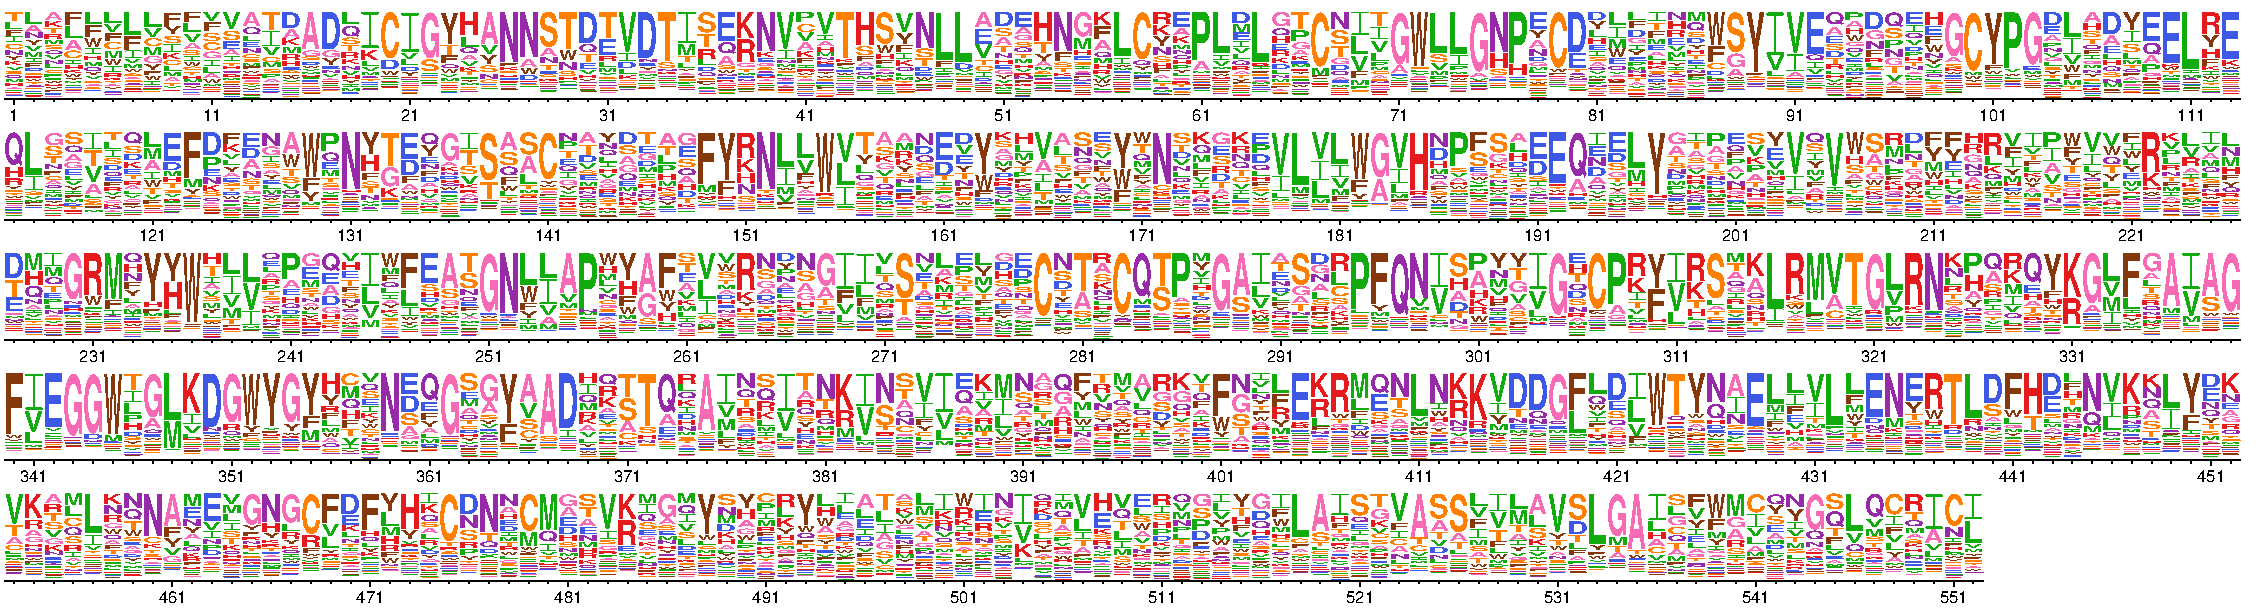
\includegraphics[width=\textwidth]{figures/prefs_doud}}
\caption{\label{suppfig:prefs_doud}
\textbf{H1 preferences measured by \cite{doud2016accurate} rescaled with the ExpCM stringency parameter optimized in \ref{fig:tree_doud}A  ($\beta = 1.19$)} 
\skhcomment{I need to change the $\beta$ value when the new \texttt{phydms} results finish running.}
}
\end{suppfig}

\begin{suppfig}[H]
\centerline{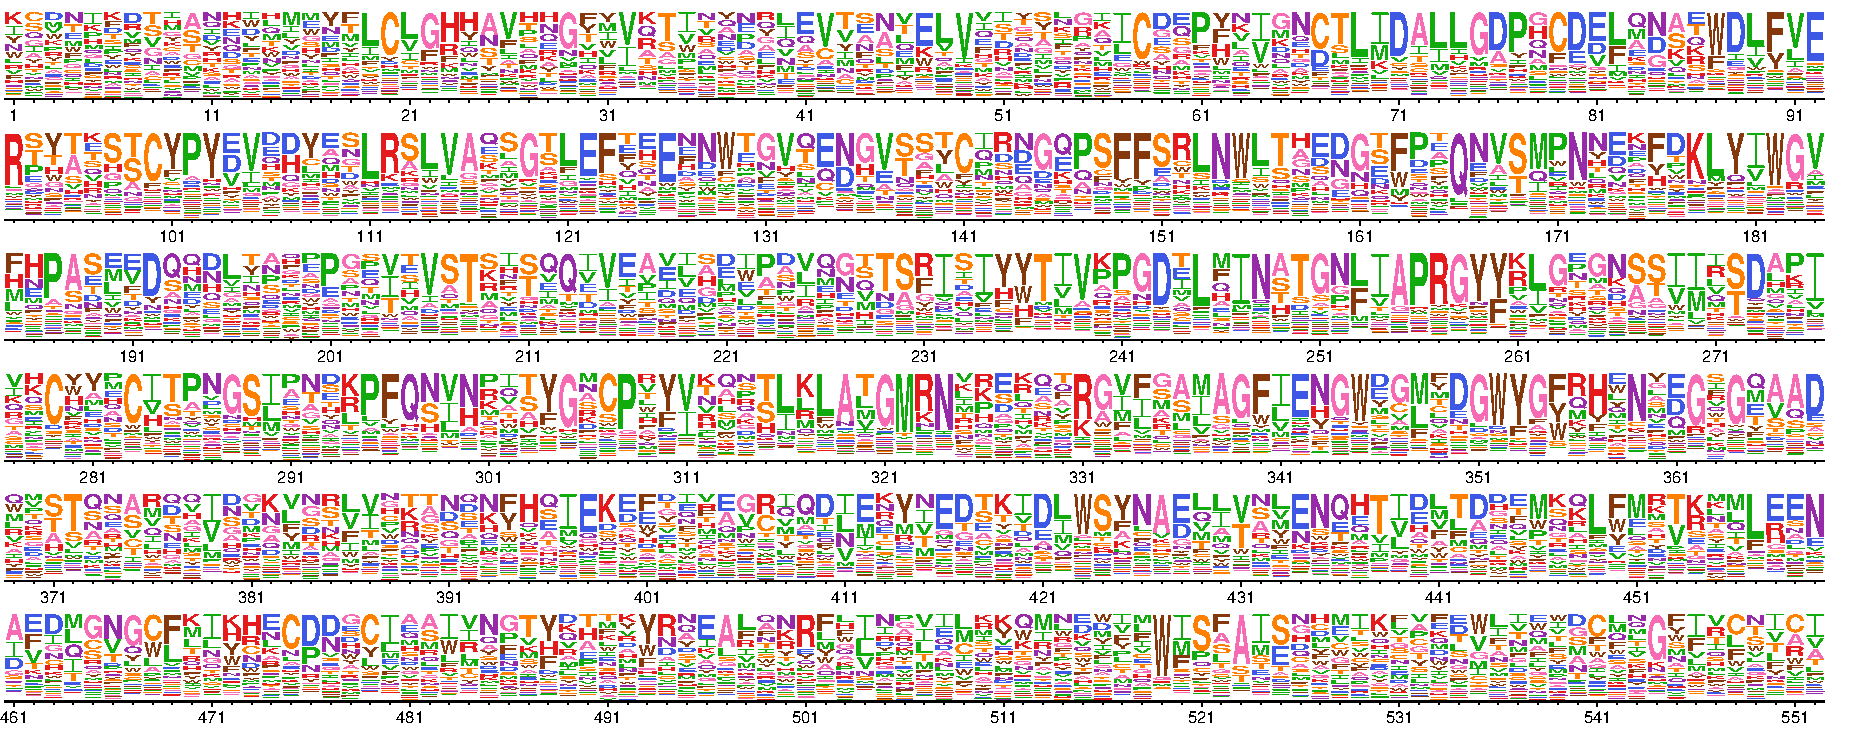
\includegraphics[width=\textwidth]{figures/prefs_lee}}
\caption{\label{suppfig:prefs_lee}
\textbf{H3 preferences measured by \textit{lee} rescaled with the ExpCM stringency parameter optimized in \ref{fig:tree_lee}A  ($\beta = 1.46$)}
 }
\end{suppfig}

\begin{suppfig}[H]
\centerline{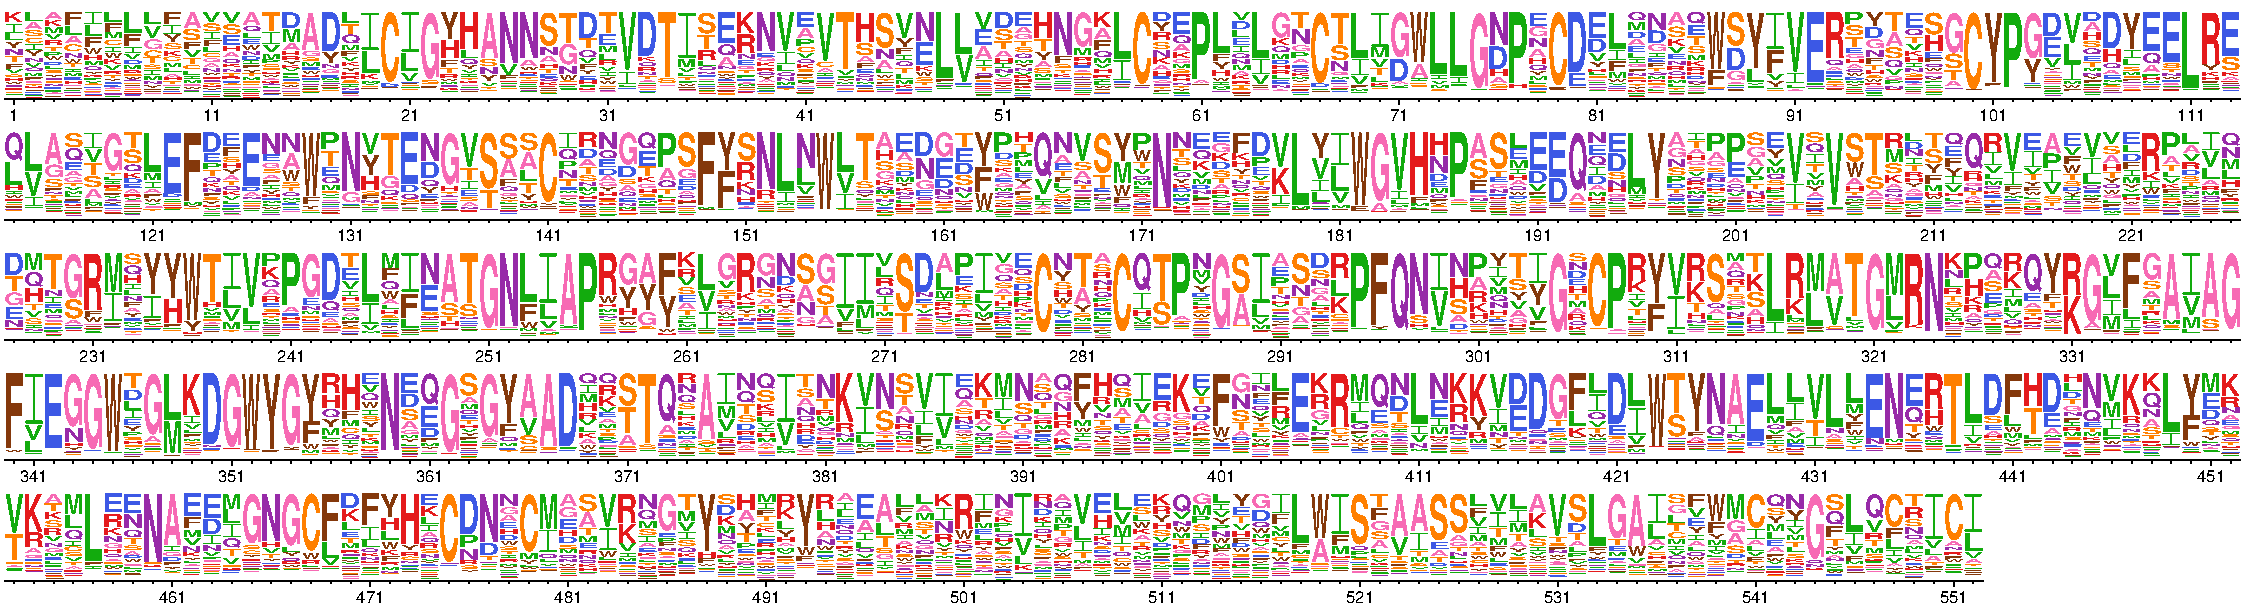
\includegraphics[width=\textwidth]{figures/prefs_average}}
\caption{\label{suppfig:prefs_average}
\textbf{The average of the H1 preferences measured by \cite{doud2016accurate} and the H3 preferences measured by \textit{Lee} rescaled with the ExpCM stringency parameter optimized in \ref{fig:tree_average}A  ($\beta = 1.77$)}}
\end{suppfig}

\begin{suppfig}[H]
\centerline{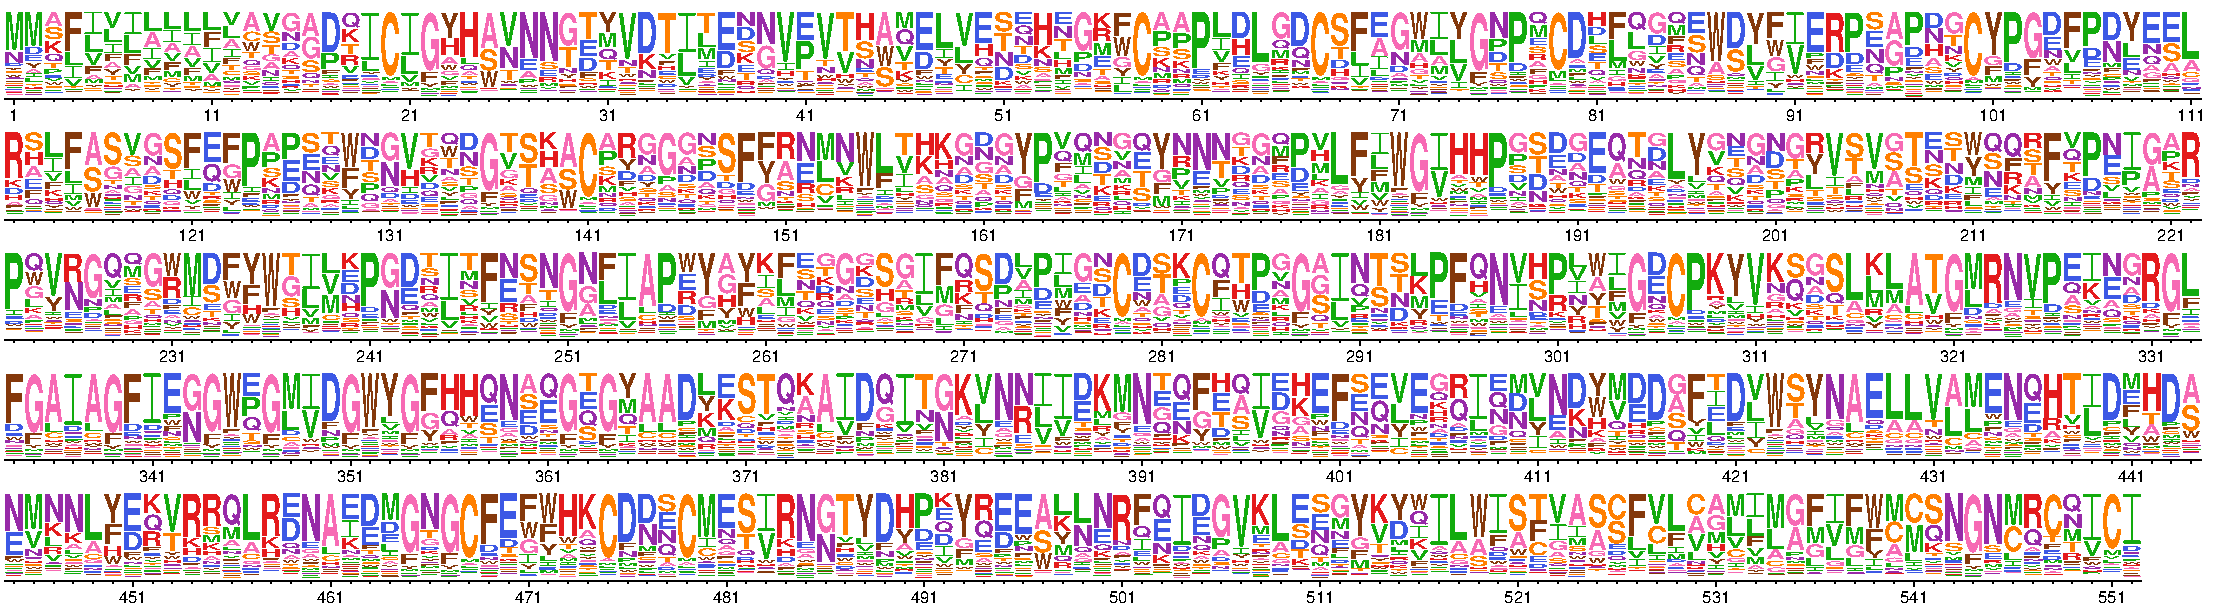
\includegraphics[width=\textwidth]{figures/prefs_mutSel}}
\caption{\label{suppfig:prefs_mutSel}
\textbf{Preferences inferred by the mutSel model on the full HA tree.}
}
\end{suppfig}


\clearpage 
\bibliographystyle{mbe}
\bibliography{references.bib}



\end{document}